\documentclass{beamer}
\usepackage{graphicx,color,amsmath,amssymb,amsfonts,amsbsy,amsthm}
% Node the following tag will orient things right using dvi2pdf.
% Process with LaTeX first, then dvi2pdf.  See GOMA docs.
\special{landscape}
% Fuzz -----------------------------------------------------------
\hfuzz5pt % Don't bother to report overfull boxes < 5pt
% MATH -----------------------------------------------------------
\input{kalman_cmdmaster.tex}
% THEOREM ENV. ---------------------------------------------------
\newtheorem{thm}{Theorem.}
\newtheorem{cor}[thm]{Corollary.}
\newtheorem{con}[thm]{Conjecture.}
\newtheorem{lem}[thm]{Lemma.}
\newtheorem{prop}[thm]{Proposition.}
\newtheorem{defn}[thm]{Definition.}
\renewcommand{\thethm}{}  % unnumbered
\pagestyle{plain}
%%% --------------------------------------------------------------
\begin{document}
\title{
\vfill \hrulefill \vfill
\begin{center}
Overview of Kalman Filter Theory and Applications\\
\end{center}
}
\author{Michael L. Carroll}
\date{July 5, 2007\\
\vfill \hrulefill \vspace*{.25in} \vfill
\begin{tiny}
\copyright 2007 by Michael L. Carroll
\end{tiny}
}
\maketitle

% ----------------------------------------------------------------
\begin{frame}
Topics\\
\begin{itemize}
  \item Control Segment Ephemeris and Clock Estimator (ECEST)
  \item ECEST State Variables
  \item ECEST Measurement Model
  \item ECEST Partitioning
\end{itemize}
\end{frame}

\begin{frame}
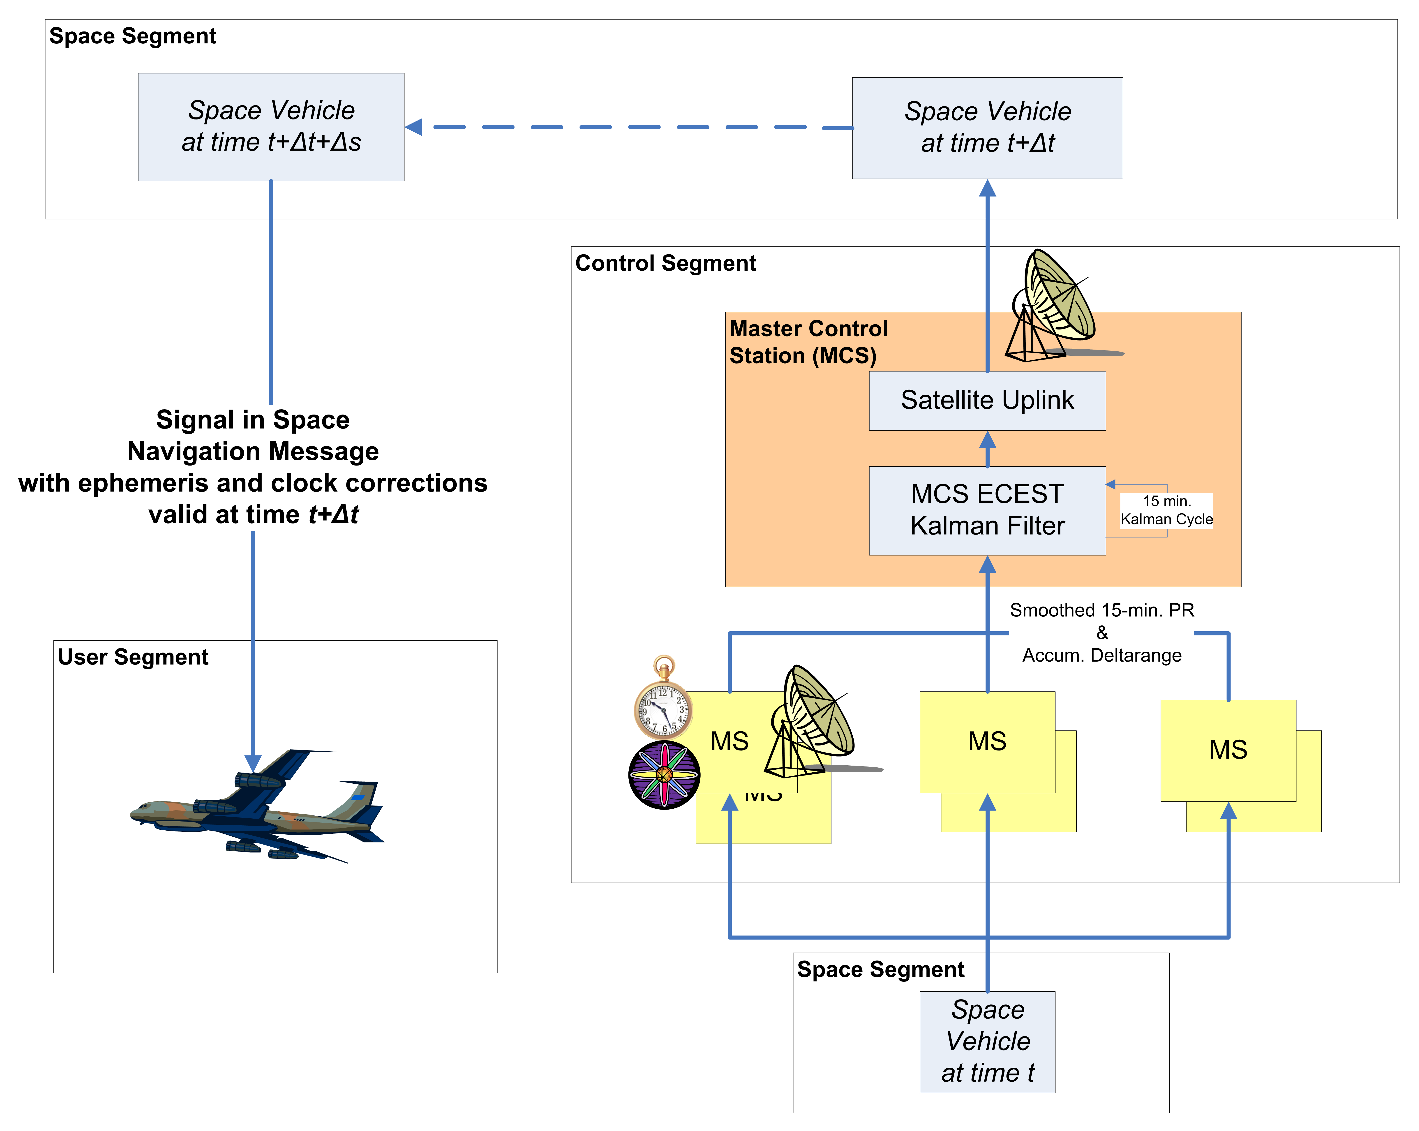
\includegraphics[scale=0.60]{cs_kalman.eps}
\end{frame}


\begin{frame}
Control Segment Ephemeris and Clock Estimator (ECEST)\\
\begin{itemize}
  \item Kalman Filter to estimate satellite ephemeris residuals and clock errors
  \begin{itemize}
     \item Inertial positions and velocities of SV
     \item SV and Monitoring Station (MS) clock biases and their derivatives 
     \item Solar pressure parameters
     \item Tropospheric state at each MS
      \end{itemize}
\end{itemize}
\end{frame}

\begin{frame}
Control Segment Ephemeris and Clock Estimator (ECEST)\\
\begin{itemize}
     \item Hundreds of state variables
     \begin{itemize}
     \item Primary variables of interest are SV position, velocity and clock errors, 
     because these are used directly by the the User Equipment
     to compute user position, velocity and time.
     \end{itemize}
     \item Partitioned into decoupled blocks based on SV-MS pairs 
\end{itemize}
\end{frame}


\begin{frame}
Residual States vs. Whole States\\
\begin{itemize}
  \item Epoch State Residual
  \item Reference Trajectory for each SV
  \item Residual is difference between reference trajectory
  and the true state
  \item Residual states sometimes called error states  
\end{itemize}
\end{frame}

\begin{frame}
ECEST State Variables -- Position\\
\begin{itemize}
  \item $\svposvec{t}=$ current position vector of the center of gravity of the SV body in Earth-centered, inertial
coordinates (meters).
  \item $\svrefposvec{t}=$ nominal (reference) position vector of the center of gravity of the SV body in Earth-centered,
inertial coordinates (meters)
  \item $\svsaposvec{t}=$ current position vector of SV antenna phase center in Earth-centered, inertial
coordinates (meters)
  \item $\msantposvec{t}=$ current position vector of MS antenna in Earth-centered, inertial coordinates (meters)
\end{itemize}
\end{frame}

\begin{frame}
ECEST State Variables -- SV and MS Antenna States\\
\begin{itemize}
  \item $\svsaposvec{t}=$ current position vector of SV antenna phase center in Earth-centered, inertial
coordinates (meters)
  \item $\msantposvec{t}=$ current position vector of MS antenna in Earth-centered, inertial coordinates (meters)
  \item $\msantphaseposvec{t}=$  current position vector of the MS antenna phase center in Earth-centered, inertial
coordinates (meters)
\end{itemize}
\end{frame}

\begin{frame}
ECEST State Variables -- Velocity States\\
\begin{itemize}
  \item $\currsvvel{t}=$ current velocity vector of the center of gravity of the SV body in Earth-centered, inertial
coordinates (meters/sec)
 \item $\refsvvel{t}=$ nominal (reference) velocity vector of the center of gravity of the SV body in Earthcentered,
inertial coordinates (meters/sec)
\end{itemize}
\end{frame}

\begin{frame}
ECEST State Variables -- Current Solar Pressure Parameters\\
\begin{itemize}
  \item $\currsolarone{t}=$ current solar pressure scaling parameter along the sunline (unitless)
  \item $\currsolartwo{t}=$ current solar pressure parameter for unmodeled acceleration in force model
(meters/$\text{sec}^2$)
\end{itemize}
Bundled as mini-state vector:
\[\text{KR}(t)=\currsolarvec{t}\]
\end{frame}

\begin{frame}
ECEST State Variables -- Nominal (reference) Solar Pressure Parameters\\
\begin{itemize}
  \item $\refsolarone{t}=$ nominal (reference)  solar pressure scaling parameter along the sunline (unitless)
  \item $\refsolartwo{t}=$ nominal (reference)  solar pressure parameter for unmodeled acceleration in force model
(meters/$\text{sec}^2$)
\end{itemize}
Also bundled as mini-state vector:
\[\text{KR}_{\text{ref}}(t)=\refsolarvec{t}\]
\end{frame}

\begin{frame}
ECEST State Variables --  Current SV Clock States\\
\begin{itemize}
  \item $\currsvclockbias{t}=$ current SV clock bias (sec)
  \item $\currsvclockdrift{t}=$ current SV clock drift (sec/sec)
  \item $\currsvclockdriftrate{t}=$ current SV  clock drift rate (sec/$\text{sec}^2$)
\end{itemize}
Bundled as a mini-state vector:
\[\tau_{\text{s}}(t)=\currsvclockstatevec{t}\]
\end{frame}

\begin{frame}
ECEST State Variables --  Nominal (reference) SV Clock States\\
\begin{itemize}
  \item $\refsvclockbias{t}=$ nominal (reference) SV clock bias (sec)
  \item $\refsvclockdrift{t}=$ nominal (reference) SV clock drift (sec/sec)
  \item $\refsvclockdriftrate{t}=$ nominal (reference) SV  clock drift rate (sec/$\text{sec}^2$)
\end{itemize}
Also bundled as a mini-state vector:
\[\tau_{\text{s,ref}}(t)=\refsvclockstatevec{t}\]
\end{frame}

\begin{frame}
ECEST State Variables --  MS Clock States\\
\begin{itemize}
  \item $\tau_m(t)=$ current MS clock bias (sec)
  \item $\dot{\tau}_m(t)=$ current MS clock drift (sec/sec)
  \item $\tau_{m,\text{ref}}(t)=$ nominal (reference) MS clock bias (sec)
  \item $\dot{\tau}_{m,\text{ref}}(t)=$ nominal (reference) MS clock drift (sec/sec)
\end{itemize}
\end{frame}

\begin{frame}
ECEST State Variables -- Tropospheric States\\
\begin{itemize}
  \item $\text{X}_\text{T}(t)=$ current wet tropospheric radial height relative to the sensor (meters)
  \item $\text{X}_{\text{T,ref}}(t)=$ nominal (reference) wet tropospheric radial height relative to the sensor (meters)
\end{itemize}
\end{frame}

\begin{frame}
ECEST State Vector Model\\
 \begin{itemize}
 \item For each SV there are 11 state variables
\[\left[ r_\text{s}, v_\text{s}, \text{KR}, \tau_\text{s} \right]\trans\]
 \item For each MS there are 3 state variables:
\[ \left[\tau_\text{m}, \text{X}_\text{T} \right]\trans\]
 \item Thus, with 30 SVs and 20 MSs we have 
\[30\times 11 + 20\times 3 = 390 \text{ possible states.}\]
 \end{itemize}
\end{frame}


\begin{frame}
ECEST Measurement Model\\
 \begin{itemize}
 \item Observations / Measurement model provided by Monitoring Stations (MSs)
 \item smoothed, corrected pseudorange ($\corrpr$)
 \item corrected, accumulated delta range ($\corradr$). 
 \item corrections are made at MCS by removal of ionospheric delay
\end{itemize}
\end{frame}

\begin{frame}
ECEST Measurement Model\\
Each MS sends via UDP:
\begin{itemize}
 \item smoothed 1.5-sec L1/L2 Pseudorange and Accumulated Delta Range 
        every 15 min (Msg 83) 
 \item local weather measurements every 15 min (Msg 81)
 \end{itemize}
Each MS also sends via UDP (but not usesd in Kalman filter):
 \begin{itemize}
   \item four 1.5-sec raw L1/L2 Pseudorange and Accumulated Delta Range
  measurements every 6 sec (Msg 80)
\end{itemize}
\end{frame}

\begin{frame}
ECEST Measurement Model\\
 \begin{itemize}
 \item Each SV-MS observation pair yields two measurements
\[\svmsmeasvec\]
 \item Each SV can be paired with as many as 10 MSs
 \item Thus, observation space can also be large (dim $\leq$  30)
\end{itemize}
\end{frame}

\begin{frame}
ECEST Partitioning\\
 \begin{itemize}
 \item To reduce the size of the state and observation spaces, a block matrix partitioning scheme is employed.
 \begin{itemize}
   \item Each partition contains up to all SVs and always contains all MS States
   \item Each SV belongs to one and only one partition at any instant of time.
   \item Each partition esimtation is independent of other partitions.
 \end{itemize}
\end{itemize}
\end{frame}




% ----------------------------------------------------------------
\end{document}
